%\documentclass[11pt]{book}
%\usepackage{palatino}
%\usepackage{amsfonts,amsmath,amssymb}
% \usepackage{graphicx}
%
%
%\ifx\pdftexversion\undefined
%    \usepackage[dvips]{graphicx}
%\else
%    \usepackage[pdftex]{graphicx}
%    \usepackage{epstopdf}
%    \epstopdfsetup{suffix=}
%\fi
%
%\usepackage{color}
%
%\begin{document}
%
%%%%%%%%%%%%%%%%%%%%%%%%%%%%%%%%%%%%%%%%
% Problem Set 3
%%%%%%%%%%%%%%%%%%%%%%%%%%%%%%%%%%%%%%%%
%
%\pagestyle{empty}
%{\noindent\bf Spring 2023 \hfill Brandon~Parmanand}
%\vskip 16pt
%\centerline{\bf University of Central Florida}
%\centerline{\bf College of Business}
%\vskip 16pt
%\centerline{\bf QMB 6911}
%\centerline{\bf Capstone Project in Business Analytics}
%\vskip 10pt
%\centerline{\bf Solutions:  Problem Set \#2}
%\vskip 32pt
%\noindent
%
\section*{Assignment Description}
% 
This assignment focuses on the analysis of the dependent variable, price with regards to whether it is owner occupied or a rental property.

%
\begin{figure}[h!]
  \centering
  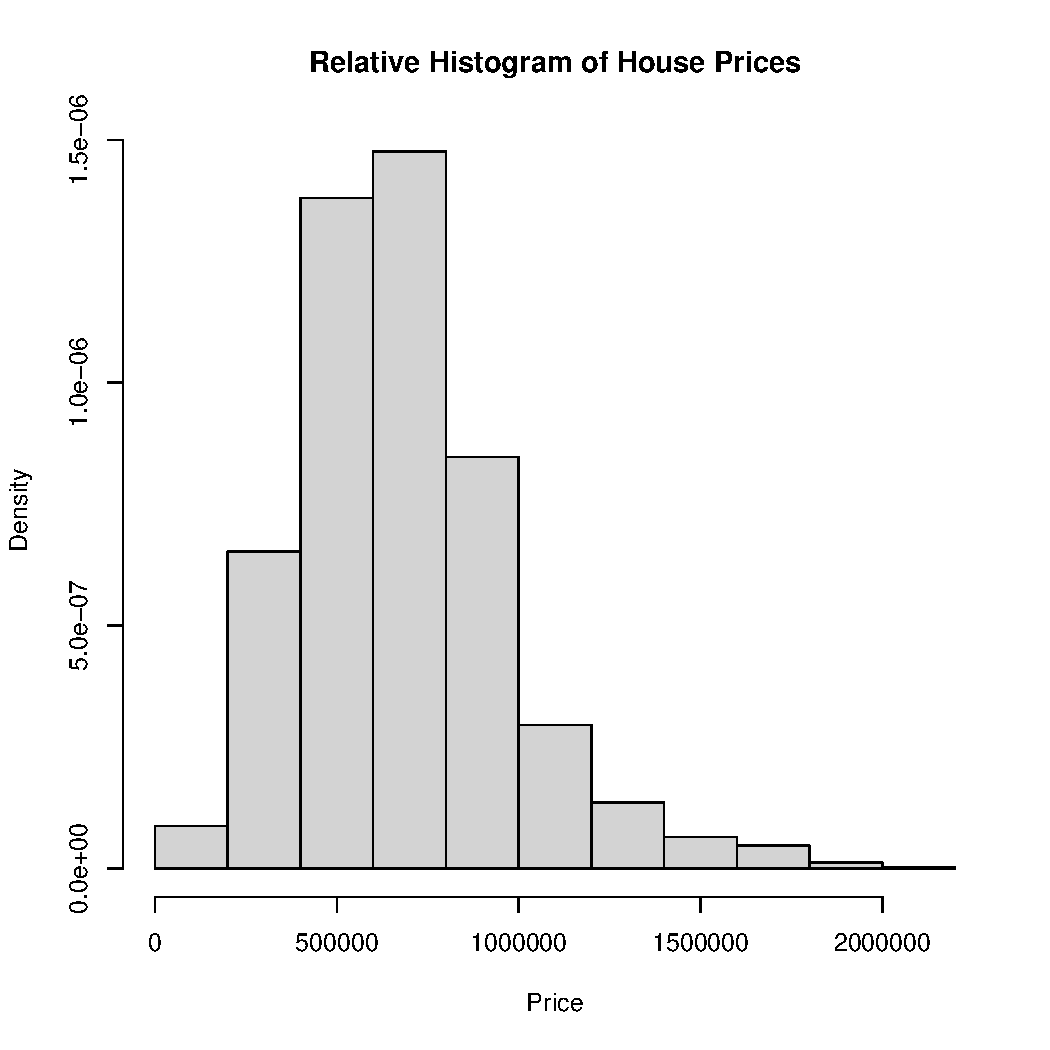
\includegraphics[scale = 0.5, keepaspectratio=true]{../Figures/hist_prices}
  \caption{Relative Histogram of House Prices} \label{fig:hist_prices}
\end{figure}
%
%
\begin{figure}[h!]
  \centering
  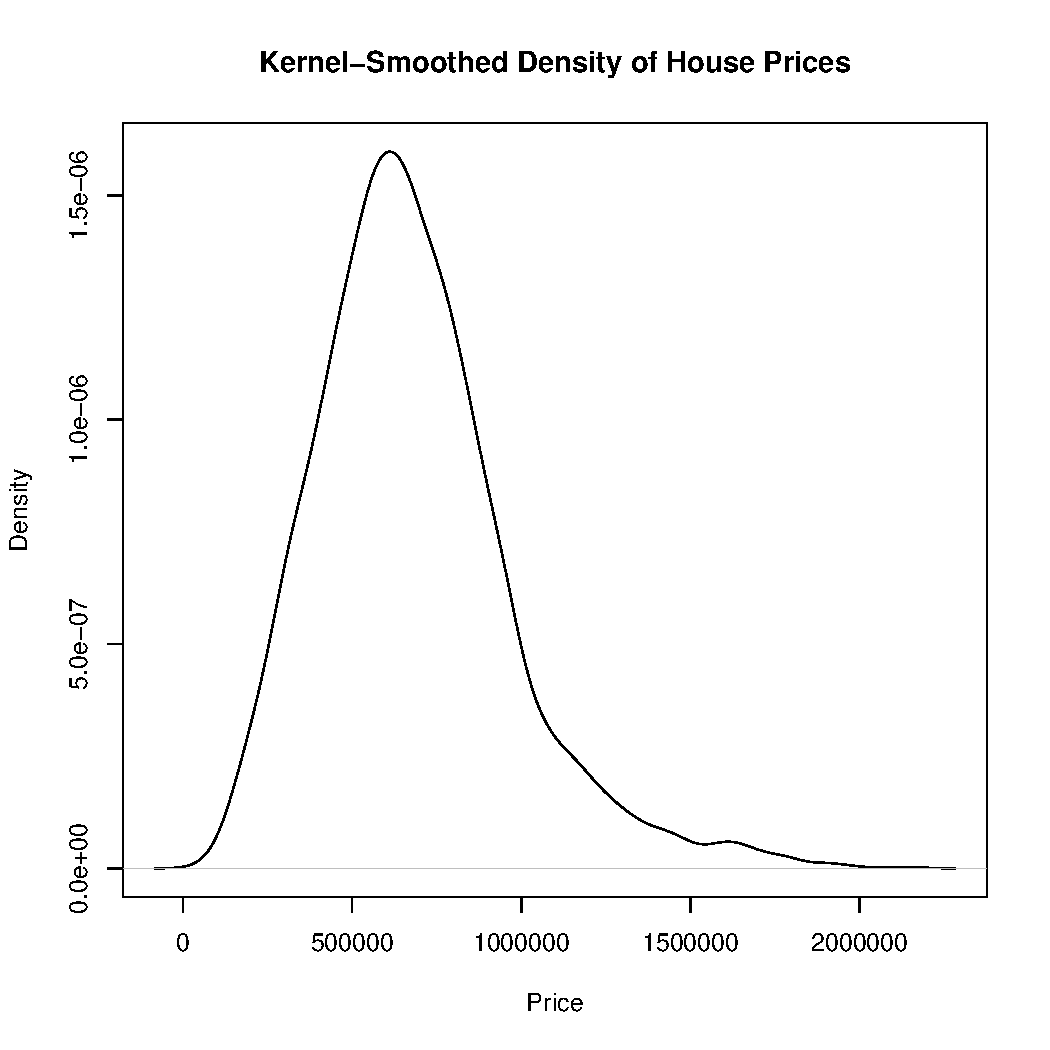
\includegraphics[scale = 0.5, keepaspectratio=true]{../Figures/density_Price}
  \caption{Relative Density of House Prices} \label{fig:density_Price}
\end{figure}
%
%

\begin{figure}[h!]
  \centering
  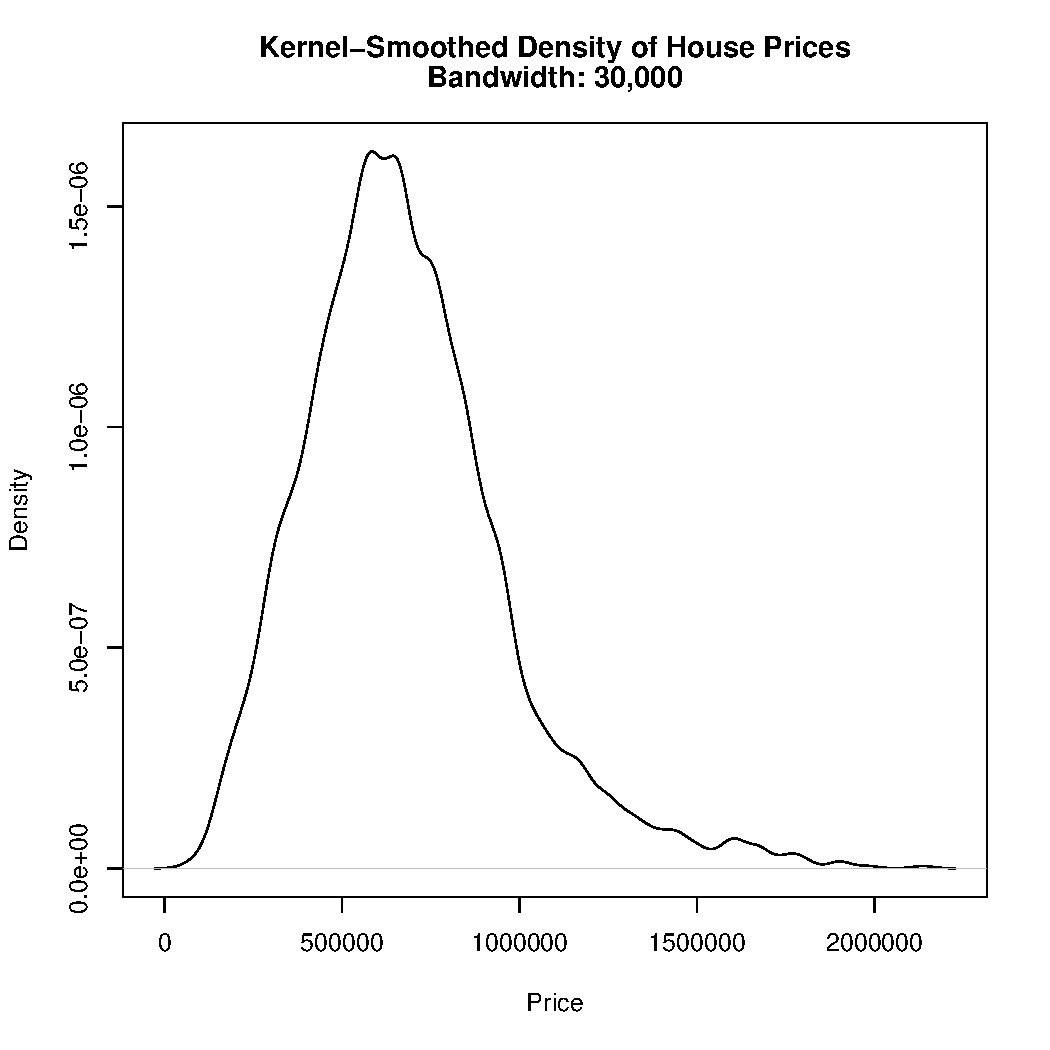
\includegraphics[scale = 0.5, keepaspectratio=true]{../Figures/density_Price_bw30000}
  \caption{Relative Density of House Prices w/ BW = 30,000} \label{fig:density_Price_bw30000}
\end{figure}
%
%
\begin{figure}[h!]
  \centering
  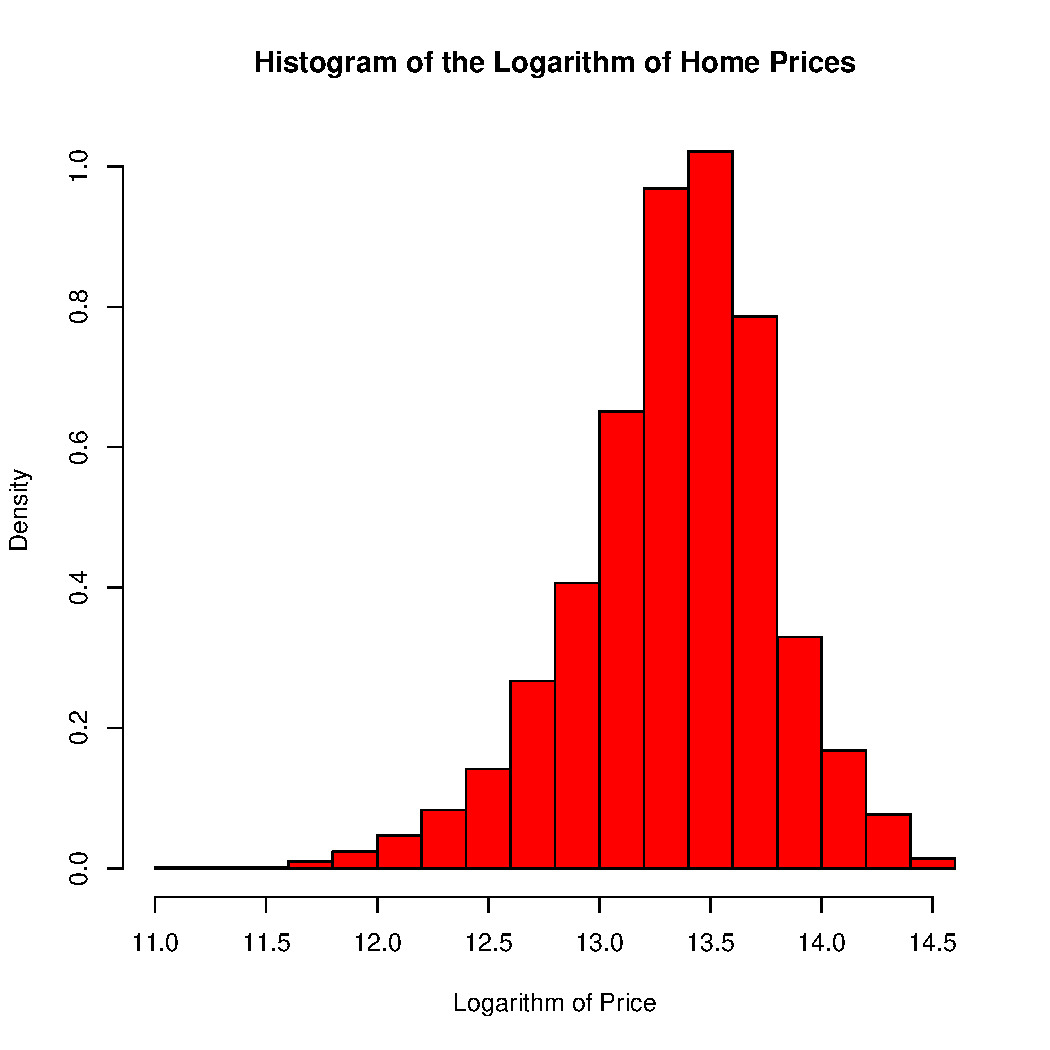
\includegraphics[scale = 0.5, keepaspectratio=true]{../Figures/hist_log_price}
  \caption{Relative Histogram of the House Log Prices} \label{fig:hist_log_price}
\end{figure}
%
%
\begin{figure}[h!]
  \centering
  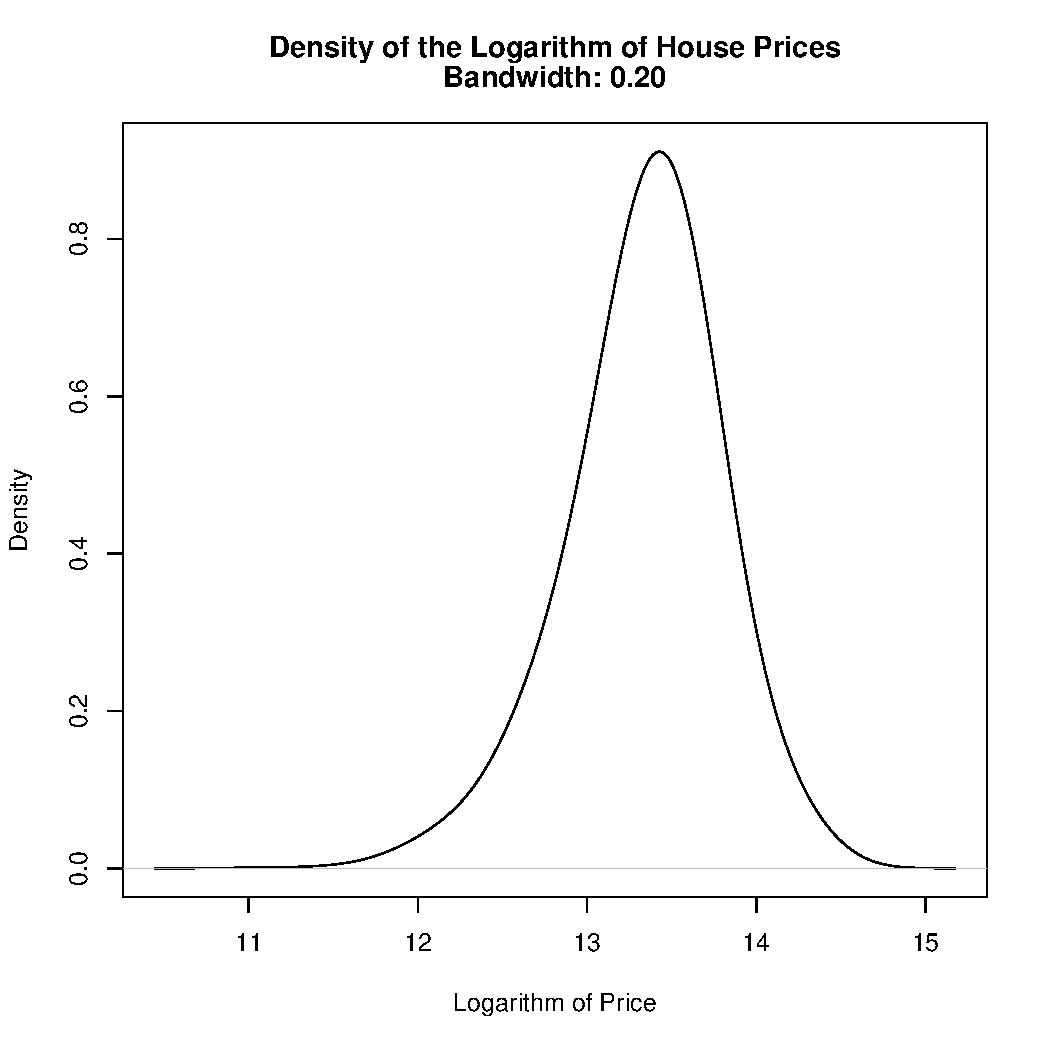
\includegraphics[scale = 0.5, keepaspectratio=true]{../Figures/density_log_saleprice_bw020}
  \caption{Relative Density of House Log Prices w/ BW=0.20} \label{fig:density_log_saleprice_bw020}
\end{figure}
%
%
\begin{figure}[h!]
  \centering
  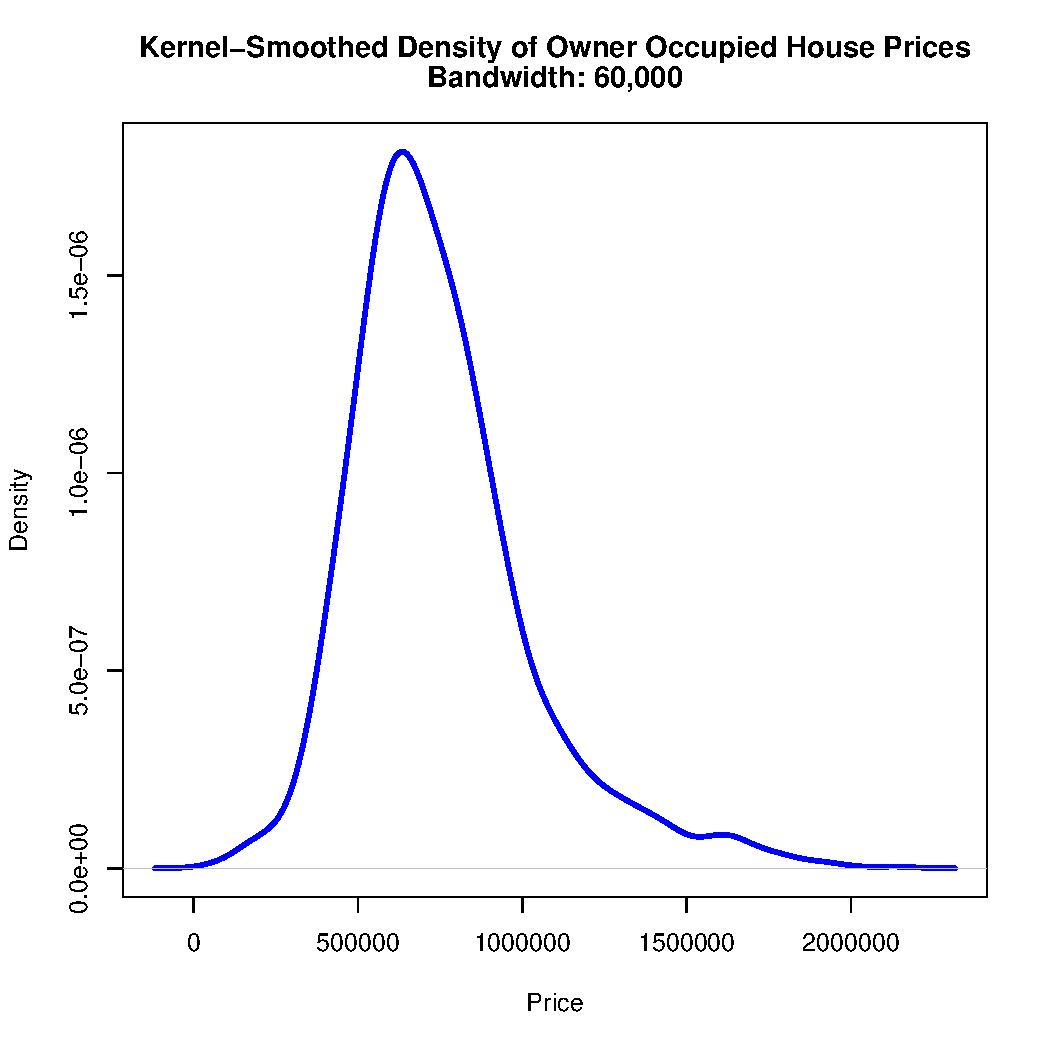
\includegraphics[scale = 0.5, keepaspectratio=true]{../Figures/density_Price_OO}
  \caption{Relative Density of Owner Occupied House Prices w/ BW=60,000} \label{fig:density_Price_OO}
\end{figure}
%
%
\begin{figure}[h!]
  \centering
  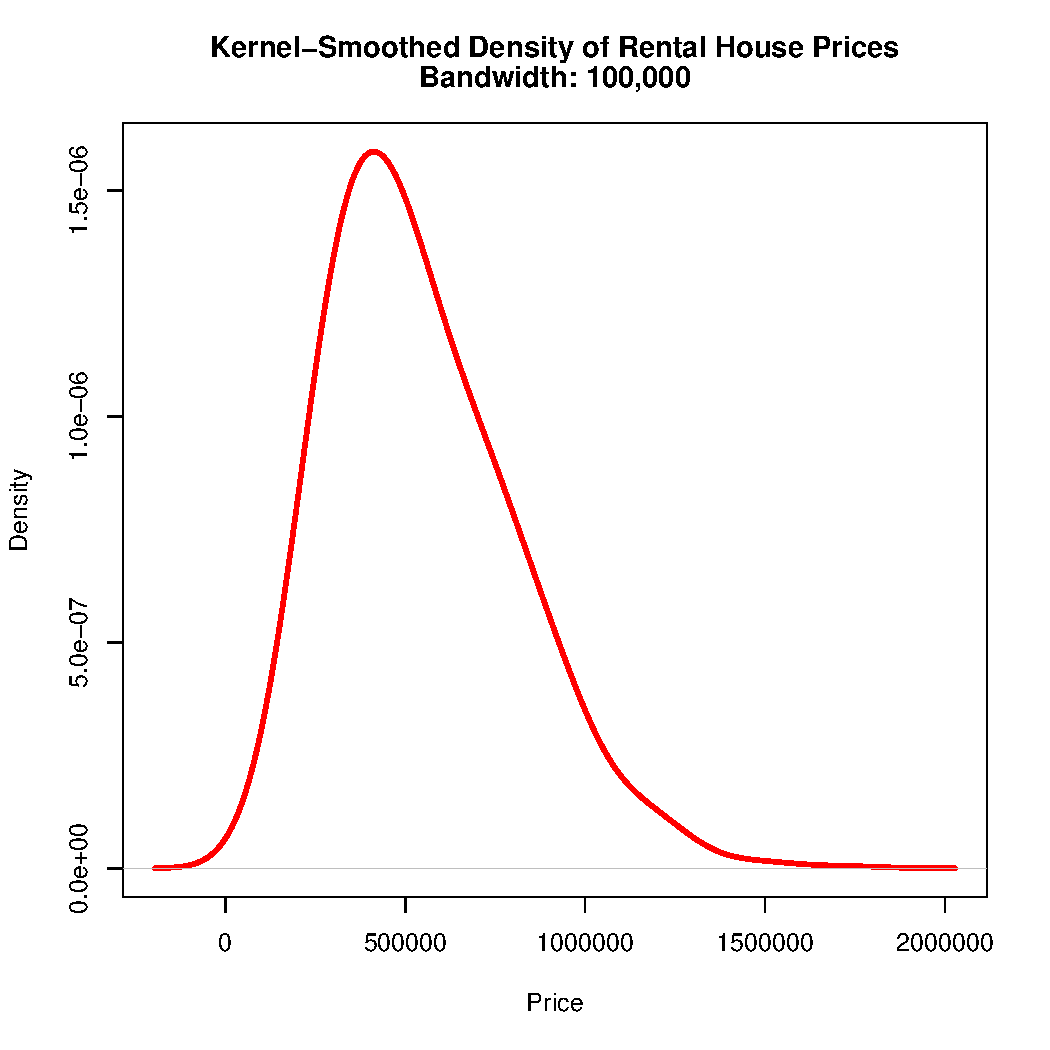
\includegraphics[scale = 0.5, keepaspectratio=true]{../Figures/density_Price_Rental}
  \caption{Relative Density of Rental House Prices w/ BW = 100,000} \label{fig:density_Price_Rental}
\end{figure}
%
%
\begin{figure}[h!]
  \centering
  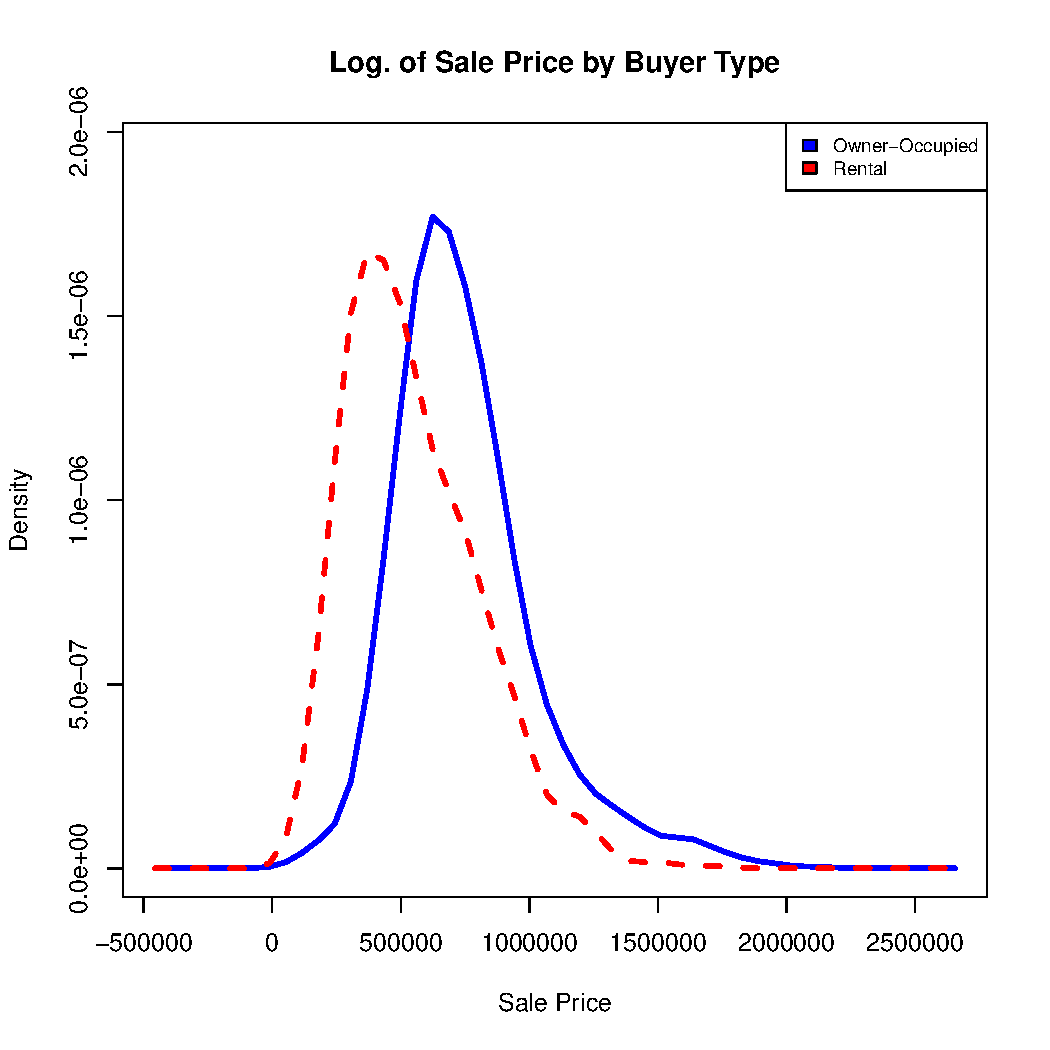
\includegraphics[scale = 0.5, keepaspectratio=true]{../Figures/dens_by_owner}
  \caption{Relative Density of House Prices of Buyer type} \label{fig:dens_by_owner}
\end{figure}
%
%
\begin{figure}[h!]
  \centering
  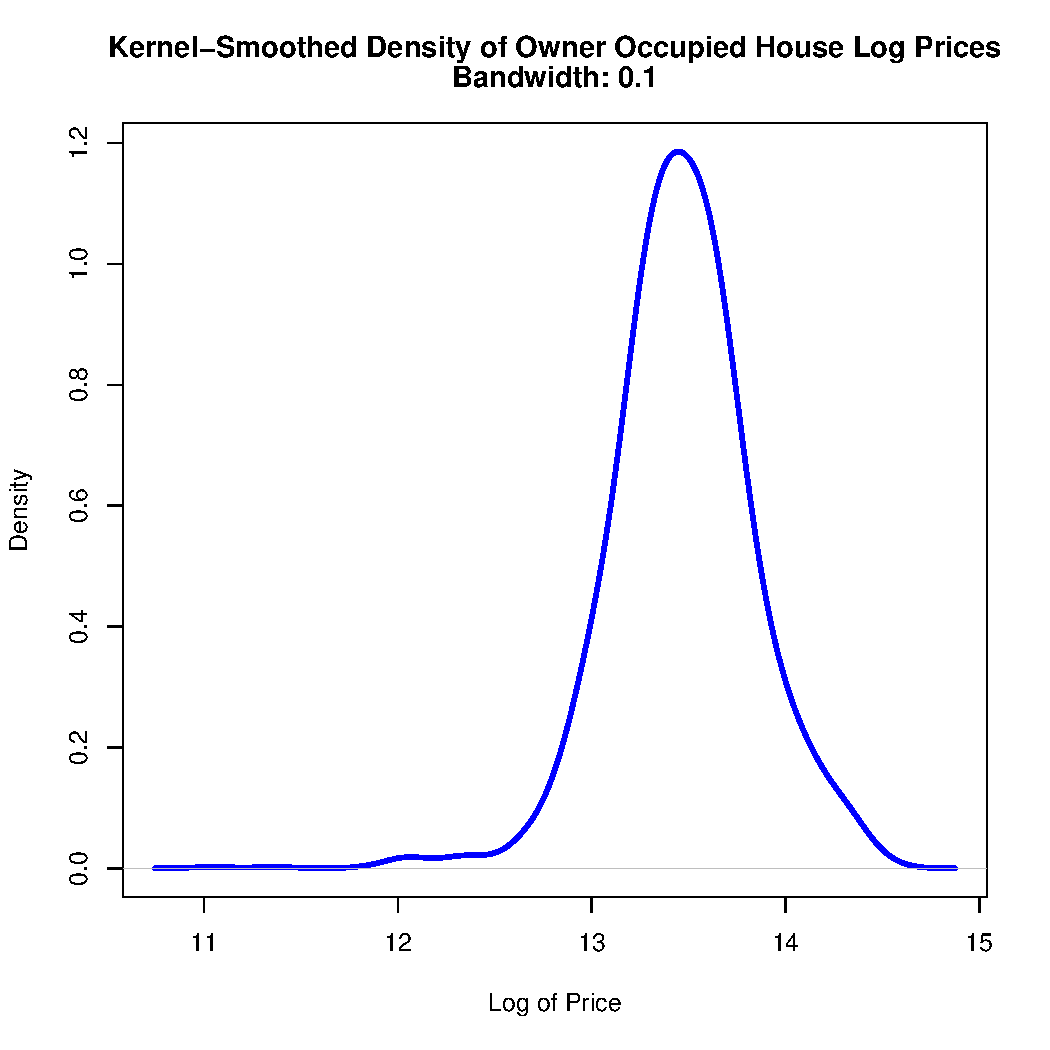
\includegraphics[scale = 0.5, keepaspectratio=true]{../Figures/log_density_Price_OO}
  \caption{Relative Density of Owner Occupied House Log Prices BW=0.1} \label{fig:log_density_Price_OO}
\end{figure}
%
%
\begin{figure}[h!]
  \centering
  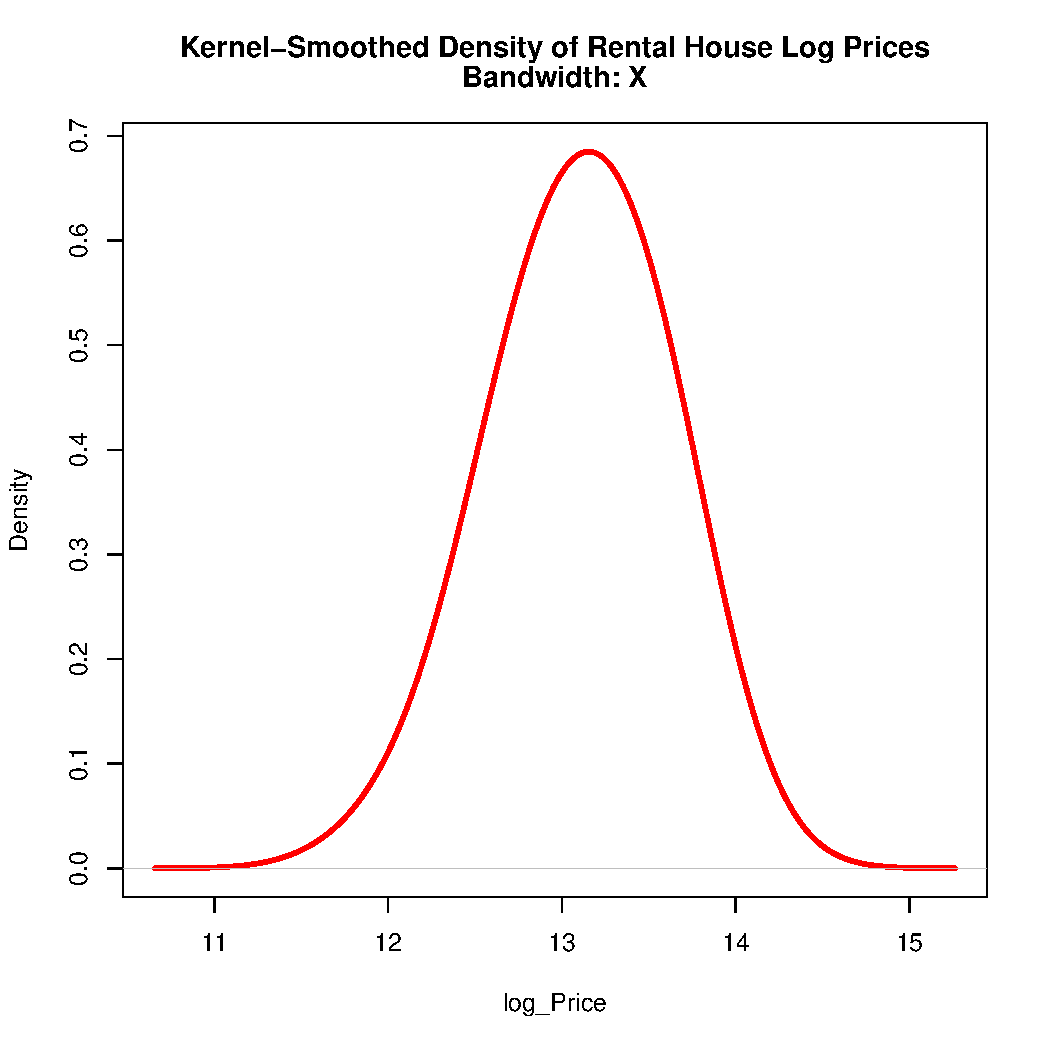
\includegraphics[scale = 0.5, keepaspectratio=true]{../Figures/log_density_Price_Rental}
  \caption{Relative Density of Rental House Log Prices BW=0.3} \label{fig:log_density_Price_Rental}
\end{figure}
%
%
\begin{figure}[h!]
  \centering
  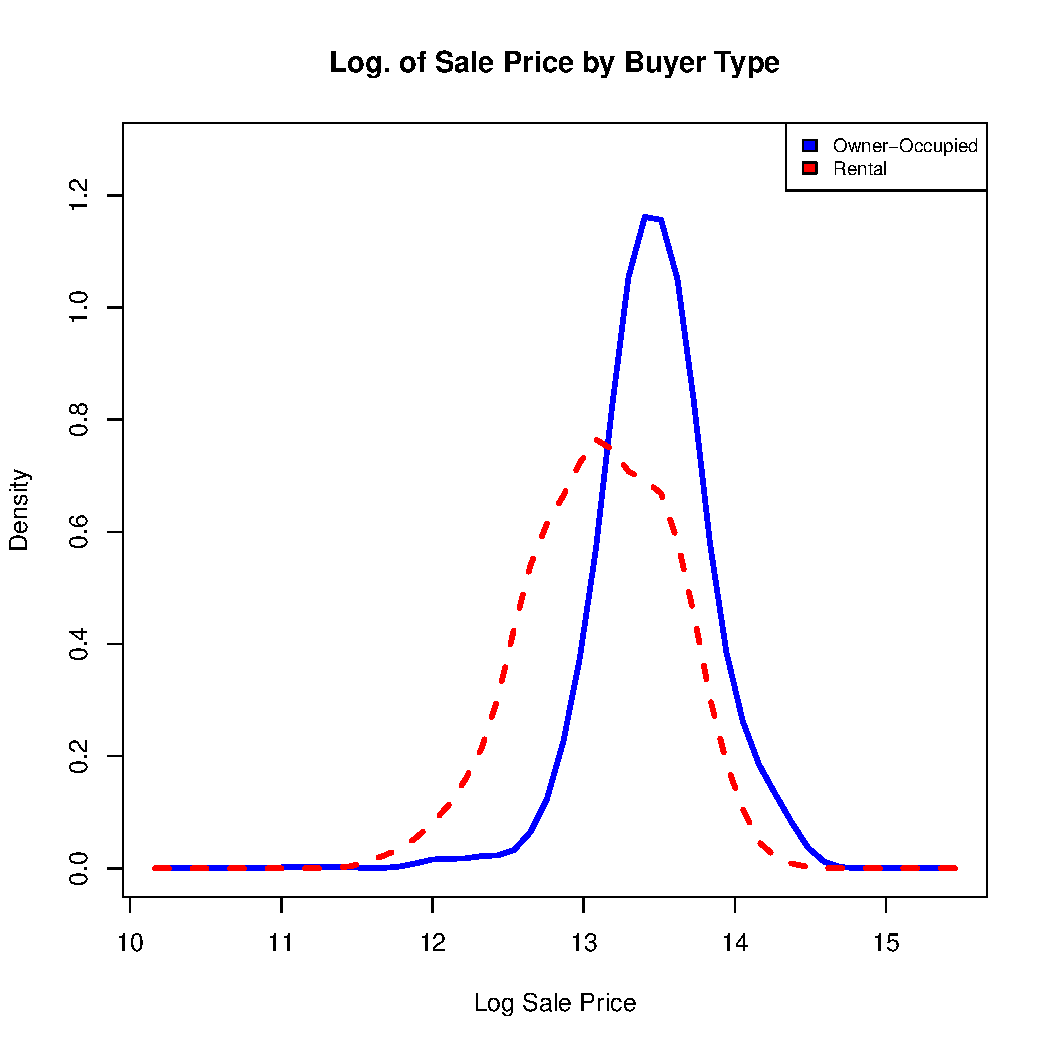
\includegraphics[scale = 0.5, keepaspectratio=true]{../Figures/log_dens_by_owner}
  \caption{Relative Density of House Log Prices of Buyer type} \label{fig:log_dens_by_owner}
\end{figure}
%
%

\bigskip
\clearpage


\begin{figure}[h!]
  \centering
  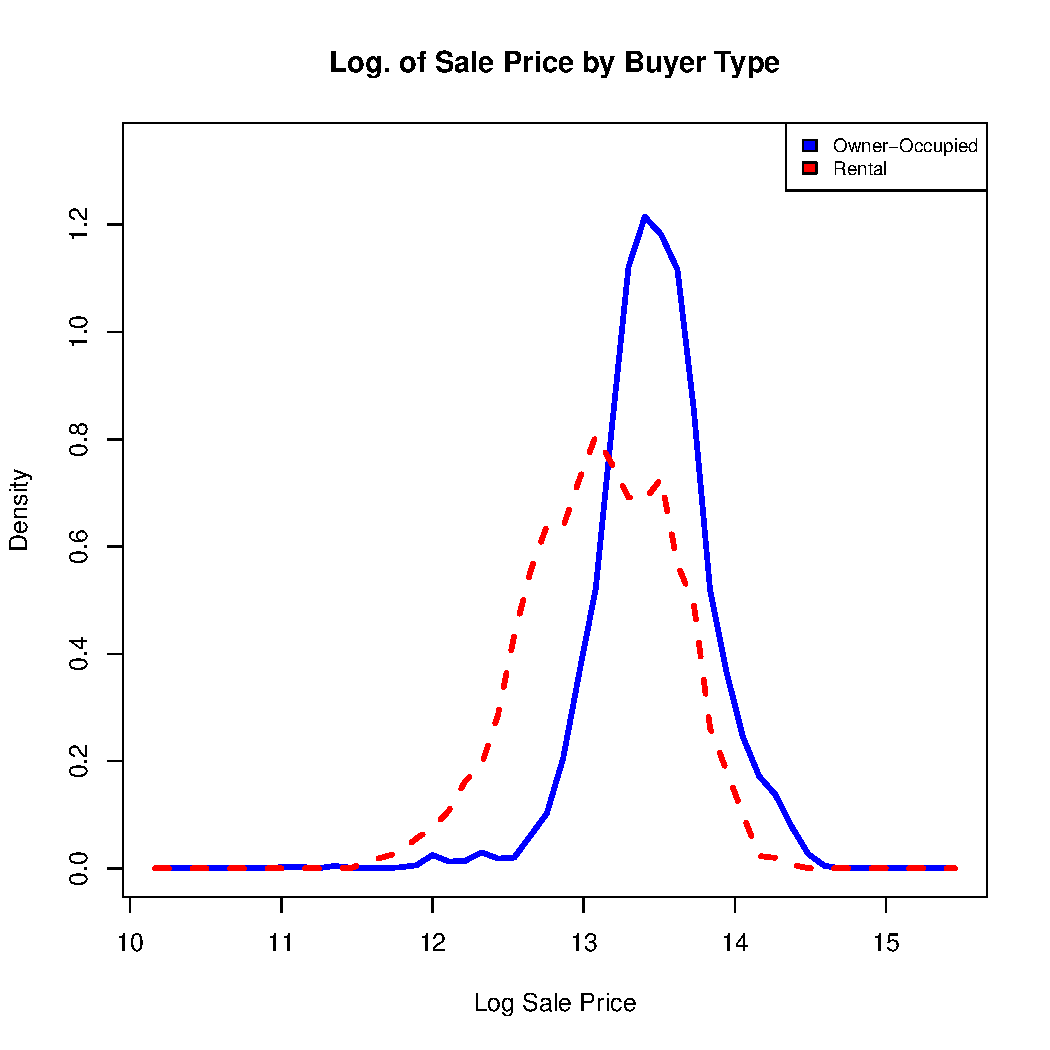
\includegraphics[scale = 0.5, keepaspectratio=true]{../Figures/log_dens_by_owner_bw}
  \caption{Relative Density of House Log Prices of Buyer type} \label{fig:log_dens_by_owner_bw}
\end{figure}


\pagebreak
When it came to adjusting the bandwidths for each Kernel-Smoothed density plot, I tried to
be careful not to over-smooth and additionally not to keep too much noise from the smaller bandwidths. Looking at the Kernel-Smoothed Density of both Owner Occupied and Rental houses.
using the natural logarithm prices, the owner-occupied houses have a bigger density than the
rental properties. Additionally, I used the bandwidth of 0.05 for owner occupied and for rental.
The rental houses prices were not as skewed as the owner-occupied ones. I do expect that the
different characteristics of homes will have different distributions relative to price and different relationships. For example, the year the house was built, or the age of the house may adversely affect the price.



%%%%%%%%%%%%%%%%%%%%%%%%%%%%%%%%%%%%%%%%
%\end{document}
%%%%%%%%%%%%%%%%%%%%%%%%%%%%%%%%%%%%%%%%
